%% ===== removed from ch4 on 2026-08-13 : fig:data:architecture =====
\begin{figure}[tb]
  \centering
  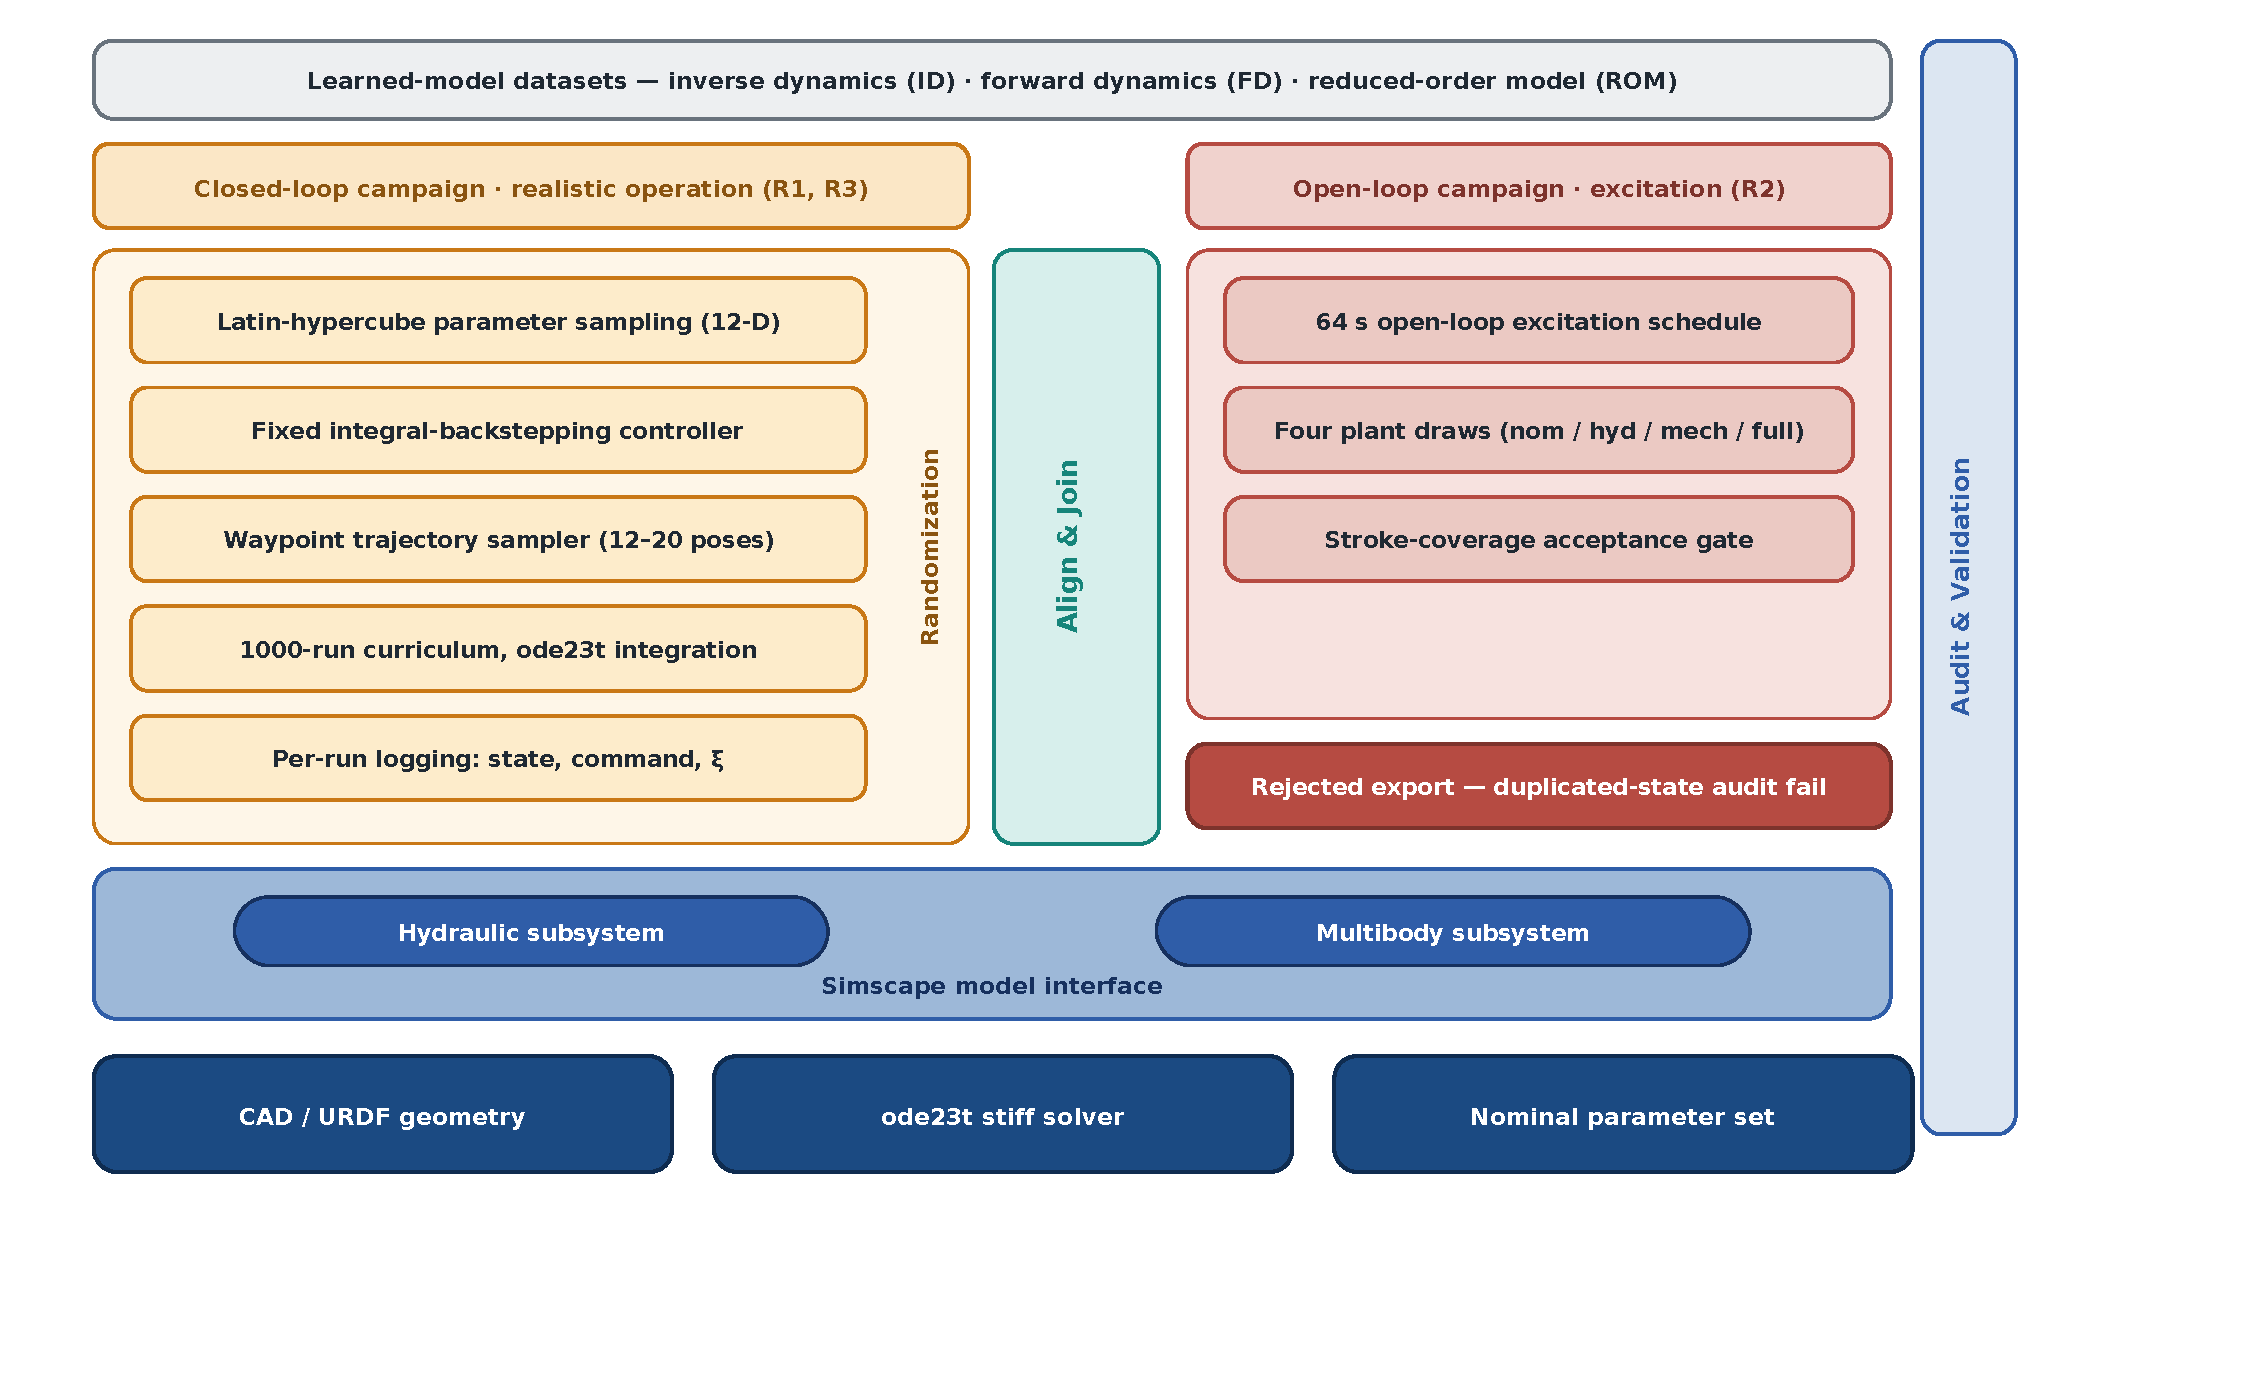
\includegraphics[width=\textwidth]{images/ch4_architecture}
  \caption{Architecture of the data-generation system. Both
  campaigns sit on the shared Simscape substrate (bottom) and feed the
  learned-model datasets (top). The closed-loop stack (left) produces realistic
  randomized operation; the open-loop stack (right) supplies the valve
  excitation that identifiability requires.}
  \label{fig:data:architecture}
\end{figure}

%% ===== removed from ch4 on 2026-08-13 : fig:data:trace =====
\begin{figure}[tb]
  \centering
  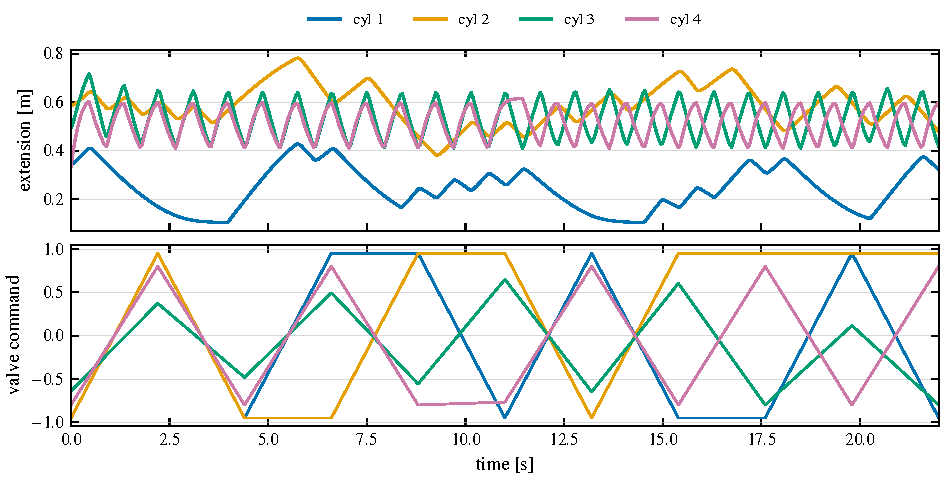
\includegraphics[width=\textwidth]{images/ch4_closed_loop_trace}
  \caption{One closed-loop operating run (fully randomized draw,
  run $601$). Top: the four cylinder extensions, moving continuously and out of
  phase as the controller tracks the waypoint trajectory. Bottom: the
  corresponding valve commands, which stay correlated with the state throughout.}
  \label{fig:data:trace}
\end{figure}

%% ===== removed prose referencing fig:data:trace =====
%Figure~\ref{fig:data:trace} shows one resulting run, a fully randomized
%draw from the second half of the curriculum. The four cylinders move
%continuously and out of phase with one another, the extensions sweep a
%large fraction of their travel, and the valve commands are the smooth
%piecewise-linear profiles that the waypoint interpolation produces
%rather than abrupt steps. This is the realistic, coordinated,
%gravity-loaded operation that requirement~R1 asks for, and it is the regime the inverse and reduced-order models are trained to be
%accurate in.
